\begin{surferPage}[Cône double]{Un Cône Double}
   Comme l'explique l'introduction de cette galerie, une surface est dite
    \emph{non--singulière} ou lisse si elle n'a pas de pointe
    (de tels points sont appelés singularités).
    Par exemple, une sphère ou un tore (les deux premières images en partant de la gauche ci-dessous):
    \begin{center}
      \begin{tabular}{@{}c@{}c@{}c@{}c@{}}
        \begin{tabular}{@{}c}
          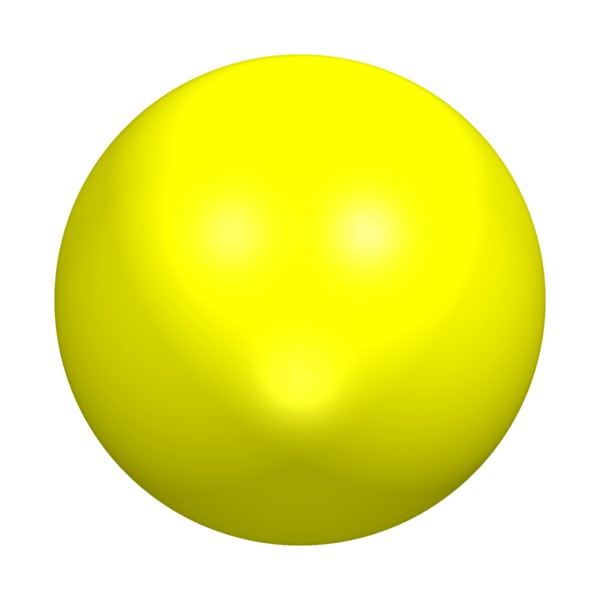
\includegraphics[width=1.4cm]{./../../common/images/kugel}
        \end{tabular}
        &
        \begin{tabular}{@{}c}
          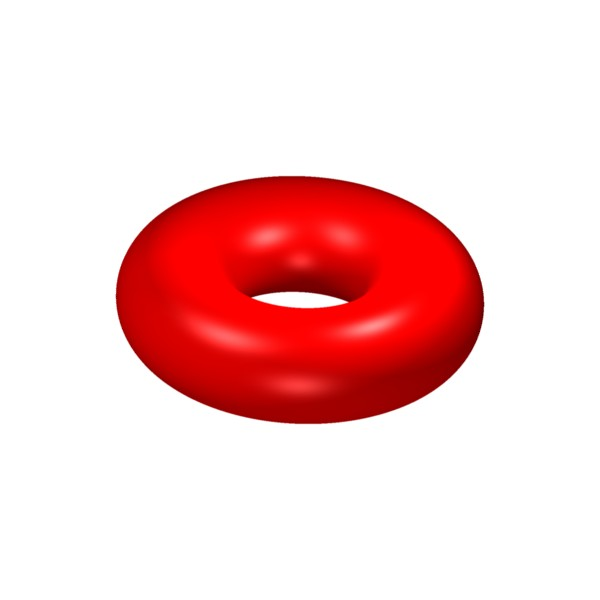
\includegraphics[width=1.4cm]{./../../common/images/torus}
        \end{tabular}
        &
        \begin{tabular}{c@{}}
          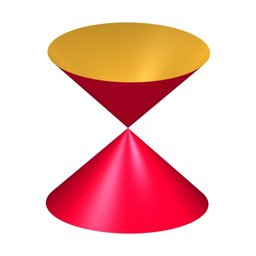
\includegraphics[width=1.4cm]{./../../common/images/kegel}
        \end{tabular}
      \end{tabular}
    \end{center}
     Le cône double (image la plus à droite) est la singularité la plus simple; c'est la seule pouvant être décrite par une équation
    de degré $2$:
    \[x^2+y^2-z^2=0.\]
    En remplaçant dans cette équation le $0$ par une valeur légèrement différente
    $a\neq 0$, le cône double devient l'un des deux types 
    d'hyperboloïdes, selon le signe de $a$:
    \begin{center}
      \begin{tabular}{@{}c@{\ }c@{\ }c@{\ }c@{\ }c@{}}
        \begin{tabular}{@{}c@{}}
          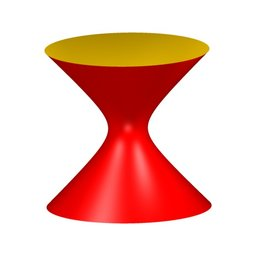
\includegraphics[width=1.2cm]{./../../common/images/A1pm_2}
        \end{tabular}
        &
        $\leftarrow$
        &
        \begin{tabular}{@{}c@{}}
          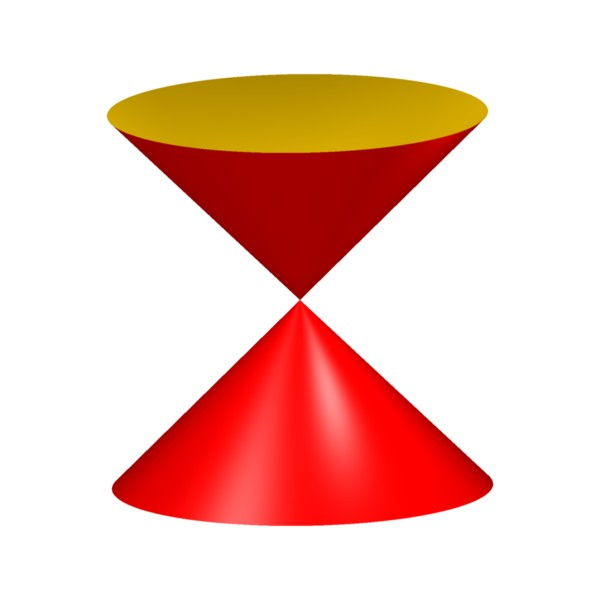
\includegraphics[width=1.2cm]{./../../common/images/A1pm_1} 
        \end{tabular}
        &
        $\rightarrow$
        &
        \begin{tabular}{@{}c@{}}
          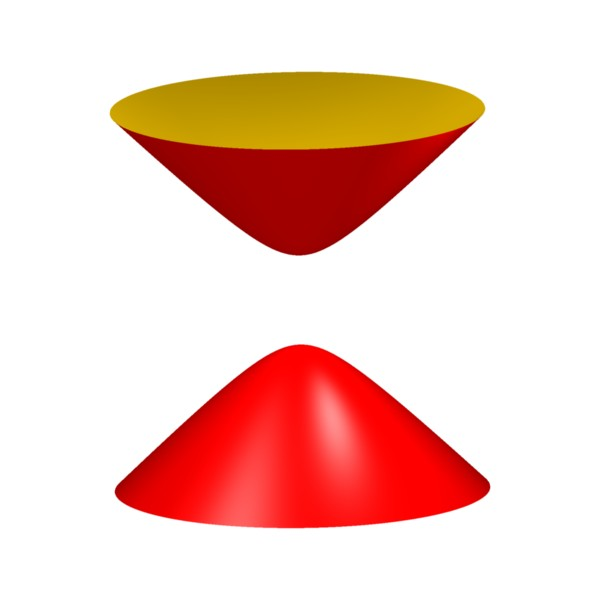
\includegraphics[width=1.2cm]{./../../common/images/A1pm_0}
        \end{tabular}
      \end{tabular}
    \end{center}
   Une surface de degré $2$ ne peut avoir au maximum qu'une singularité, soit\ $\mu(2)=1$.
\end{surferPage}
